\documentclass[border=.1cm]{standalone}

\usepackage{tikz}
\usepackage{pgfplots}
\usepgflibrary{arrows}

\usepackage{siunitx}
\sisetup{
    detect-all = true,
    input-decimal-markers = {.},
    input-ignore = {,},
    inter-unit-product = \ensuremath{{}\cdot{}},
    multi-part-units = repeat,
    number-unit-product = \text{~},
    per-mode = fraction,
    separate-uncertainty = true,
}

\begin{document}

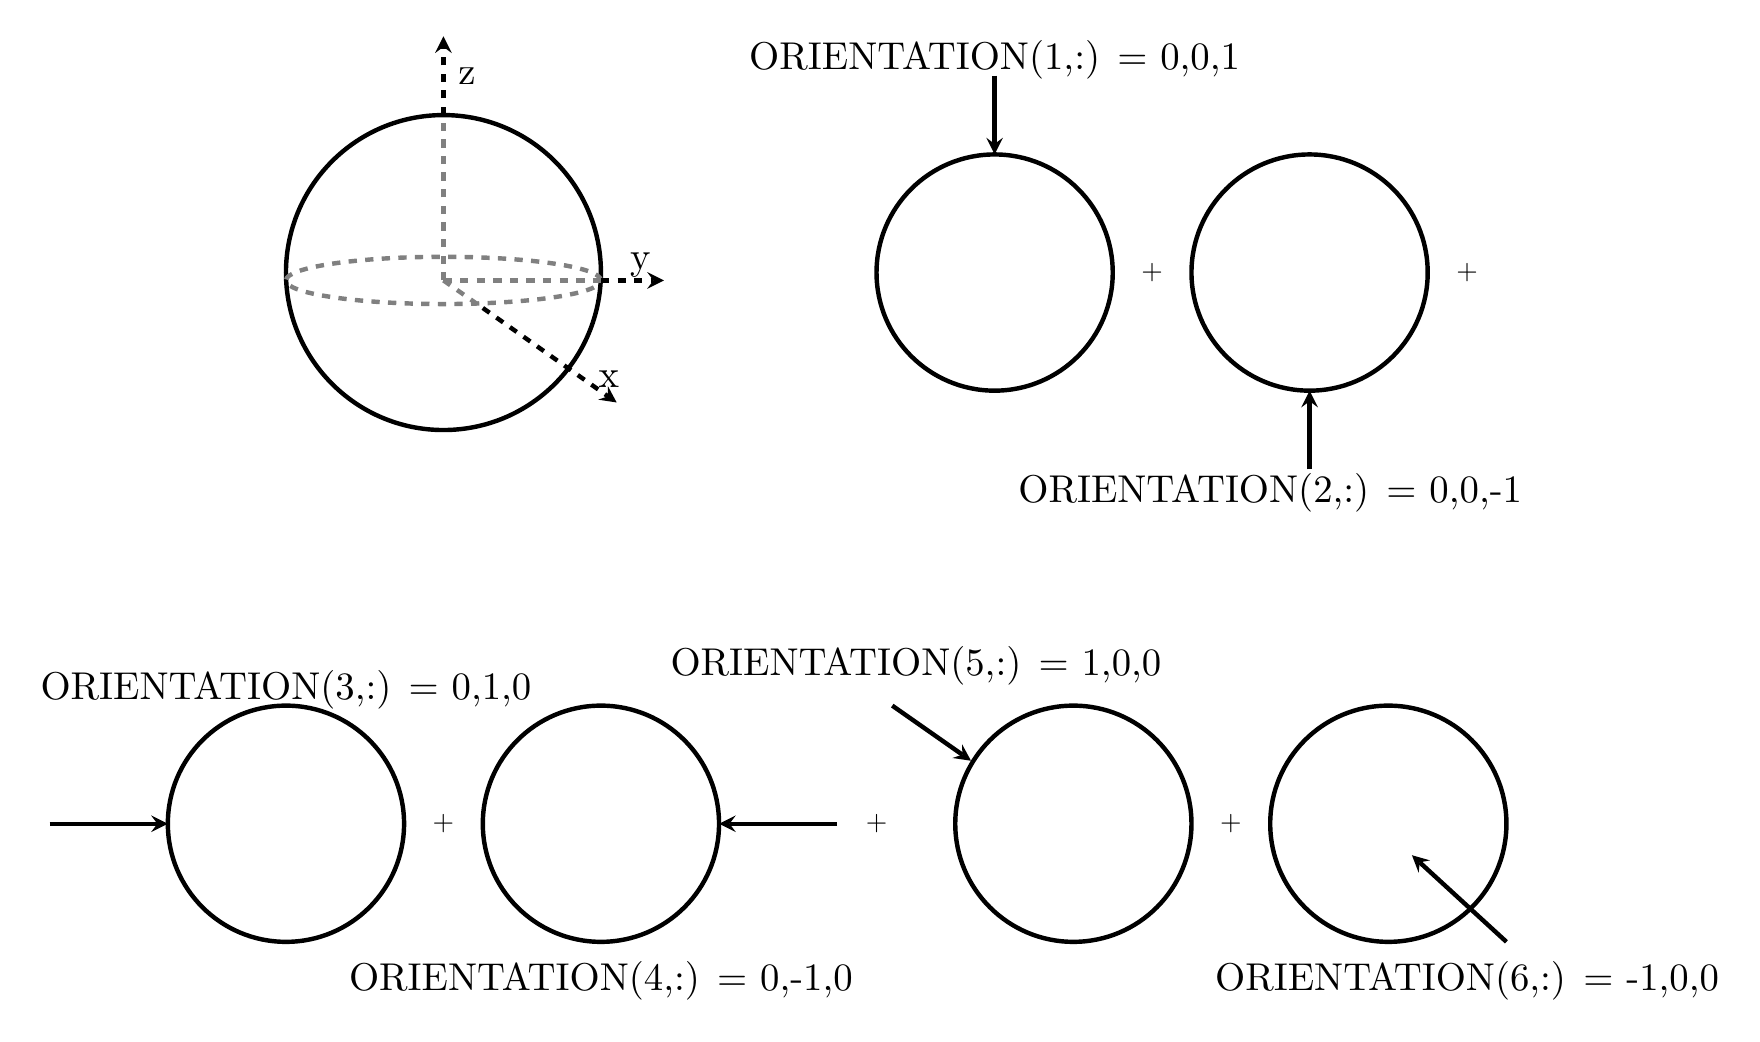
\begin{tikzpicture}

\draw [ultra thick](0,0) circle (1.5cm); 
\node at (0, 1.7)[ultra thick,scale = 1.4]{ORIENTATION(3,:) = 0,1,0}; 
\draw[-stealth,ultra thick](-3,0) -- (-1.5,0); 

\node at (2,0){+}; 

\draw [ultra thick](4,0) circle (1.5cm); 
\node at (4, -2)[ultra thick,scale = 1.4]{ORIENTATION(4,:) = 0,-1,0}; 
\draw[-stealth,ultra thick](7,0) -- (5.5,0);  

\node at (7.5,0){+}; 

\draw [ultra thick](10,0) circle (1.5cm); 
\node at (8,2)[ultra thick,scale = 1.4]{ORIENTATION(5,:) = 1,0,0}; 
\draw[-stealth,ultra thick](7.7,1.5) -- (8.7,.8);   
 
\node at (12,0){+}; 

\draw [ultra thick](14,0) circle (1.5cm); 
\node at (15,-2)[ultra thick,scale = 1.4]{ORIENTATION(6,:) = -1,0,0}; 
\draw[-stealth,ultra thick](15.5,-1.5) -- (14.3,-.4);    

\draw [ultra thick](9,7) circle (1.5cm); 
\node at (9,9.7)[ultra thick,scale = 1.4]{ORIENTATION(1,:) = 0,0,1}; 
\draw[-stealth,ultra thick](9,9.5) -- (9,8.5);    

\node at (11,7){+}; 
 
\draw [ultra thick](13,7) circle (1.5cm); 
\node at (12.5,4.2)[ultra thick,scale = 1.4]{ORIENTATION(2,:) = 0,0,-1}; 
\draw[-stealth,ultra thick](13,4.5) -- (13,5.5);     

\node at (15,7){+}; 

\draw [ultra thick](2,7) circle (2cm);  
\draw[gray,dashed,ultra thick](2,6.9) ellipse(2cm and .3cm); 
\draw[gray,dashed,ultra thick](2,6.9) -- (4,6.9); 
\draw[-stealth,dashed,ultra thick](4,6.9) -- (4.8,6.9); 
\node at (4.5,7.1)[ultra thick,scale = 1.4]{y}; 
\draw[gray,dashed,ultra thick](2,6.9) -- (2.5, 6.55); 
\draw[-stealth,dashed,ultra thick](2.5,6.55) -- (4.2, 5.35); 
\node at (4.1,5.65)[ultra thick,scale = 1.4]{x}; 
\draw[gray, dashed, ultra thick](2,6.9) -- (2,9.0);   
\draw[-stealth,dashed, ultra thick](2,9.0) -- (2,10); 
\node at (2.3,9.5)[ultra thick,scale = 1.4]{z};





\end{tikzpicture}

\end{document}